\chapter{The Multiplicative Model}\label{Chapter:MultiplicativeModel}

\newthought{One of the most famous statistical aphorisms} is due to Prof.\ George Box\cite{StatisticsForExperimenters}:
\begin{quotation}
The most that can be expected from any model is that it can supply a useful approximation to reality:

\textbf{All models are wrong; some models are useful.}
\end{quotation}
In line with this idea, in this chapter we will discuss the most important and illuminating models for SAR data that generalize the one for textureless data.

The Multiplicative Model is just one of the infinitely many ways to build stochastic descriptions for SAR data.
Among its advantages we would like to mention that it can be considered an \textit{ab initio} model, and that it leads to expressive and tractable descriptions of the data.

Let us recall that the basic model for multilook intensity data is the $\Gamma(\sigma^2,L)$ law whose density is
\begin{equation}
f_Z(z;L,\sigma^2) = \frac{L^L}{\sigma^{2L}\Gamma(L)} z^{L-1} 
	\exp\big\{ -L z / \sigma^2
	\big\}.
\end{equation}
As previously said, the Gamma distribution is scale-invariant, so we may pose this model as the product between the constant backscatter $X=\sigma^2$ and the multilook speckle $Y\sim\Gamma(1,L)$.

But, are there situations were we cannot assume a constant backscatter?
Yes, there are.

A constant backscatter results from infinitely many elementary backscatterers, i.e.\ from the assumption that $N\to\infty$ in~\eqref{Eq:ComplexBackscatter} (page~\pageref{Eq:ComplexBackscatter}).
Such assumption makes the particular choice of the sensed area irrelevant.
But this may not be the case always.

The advent of higher resolution sensors makes this hypothesis unsuitable in areas where the elementary backscatterers are of the order of the wavelength; cf.\ Table~\ref{Tab:Bands}.
If, for instance, we are dealing with a \SI{1x1}{\meter} resolution image, we may consider $N\to\infty$ if the target is flat and composed of grass;
but if the target is a forest, this assumption may be unrealistic.

\section{The $\mathcal K$ distribution}

\citet{JakemanPusey76} were among the first who tackled this problem.
Assuming that the number of elementary backscatterers $N$ fluctuates according to a Negative Binomial distribution (see Section~\ref{Sec:NegativeBinomial}), they obtained a closed-form density which characterizes the $\mathcal K$ distribution:
\begin{equation}
f_Z(z;\alpha,\lambda,L) =
\frac{2\lambda L}{\Gamma(\alpha)\Gamma(L)} (\lambda L z)^{\frac{\alpha+L}{2}-1} K_{\alpha-L}(2\sqrt{\lambda L z}),
\label{Eq:DensKI}
\end{equation}
where $\alpha>0$ measures the roughness, $\lambda>0$ is a scale parameter, and $K_\nu$ is the modified Bessel function of order $\nu$.
This special function is given by $K_\nu (z) = \int_0^\infty e^{-z} \cosh (\nu t) dt$.
See the book by \citet{Gradshteyn80} for other definitions and important properties.
This function is implemented in many numerical platforms as, for instance, in \texttt R.

We denote $Z\sim \mathcal K(\alpha,\lambda,L)$ the situation of $Z$ following the distribution characterized by~\eqref{Eq:DensKI}.
The $k$-order moments of $Z$ are
\begin{equation}
E(Z^k) = (\lambda L)^{-k} \frac{\Gamma(L+k)\Gamma(\alpha+k)}{\Gamma(L)\Gamma(\alpha)}.
\label{Eq:MomentKI}
\end{equation}
Eq.~\eqref{Eq:MomentKI} is useful, among other applications, for finding $\lambda^*=\alpha$, the scale parameter that yields a unitary mean distribution for each $\alpha$ and any $L$.

Fig.~\ref{Fig:KIDistribution} shows the densities in linear and semilogarithmic scales of the Exponential and $\mathcal K$ distributions.
They all have unitary mean, and the latter is shown with different degrees of roughness ($\alpha\in\{1,3,8\}$).
It is noticeable that the larger the value of $\alpha$ is, the closer the $\mathcal K$ and $\text{E}$ densities become.
In fact, \citet{frery96} prove that there is convergence in distribution of the latter to the former.

\begin{figure}[hbt]
\centering
\subfloat[Densities]{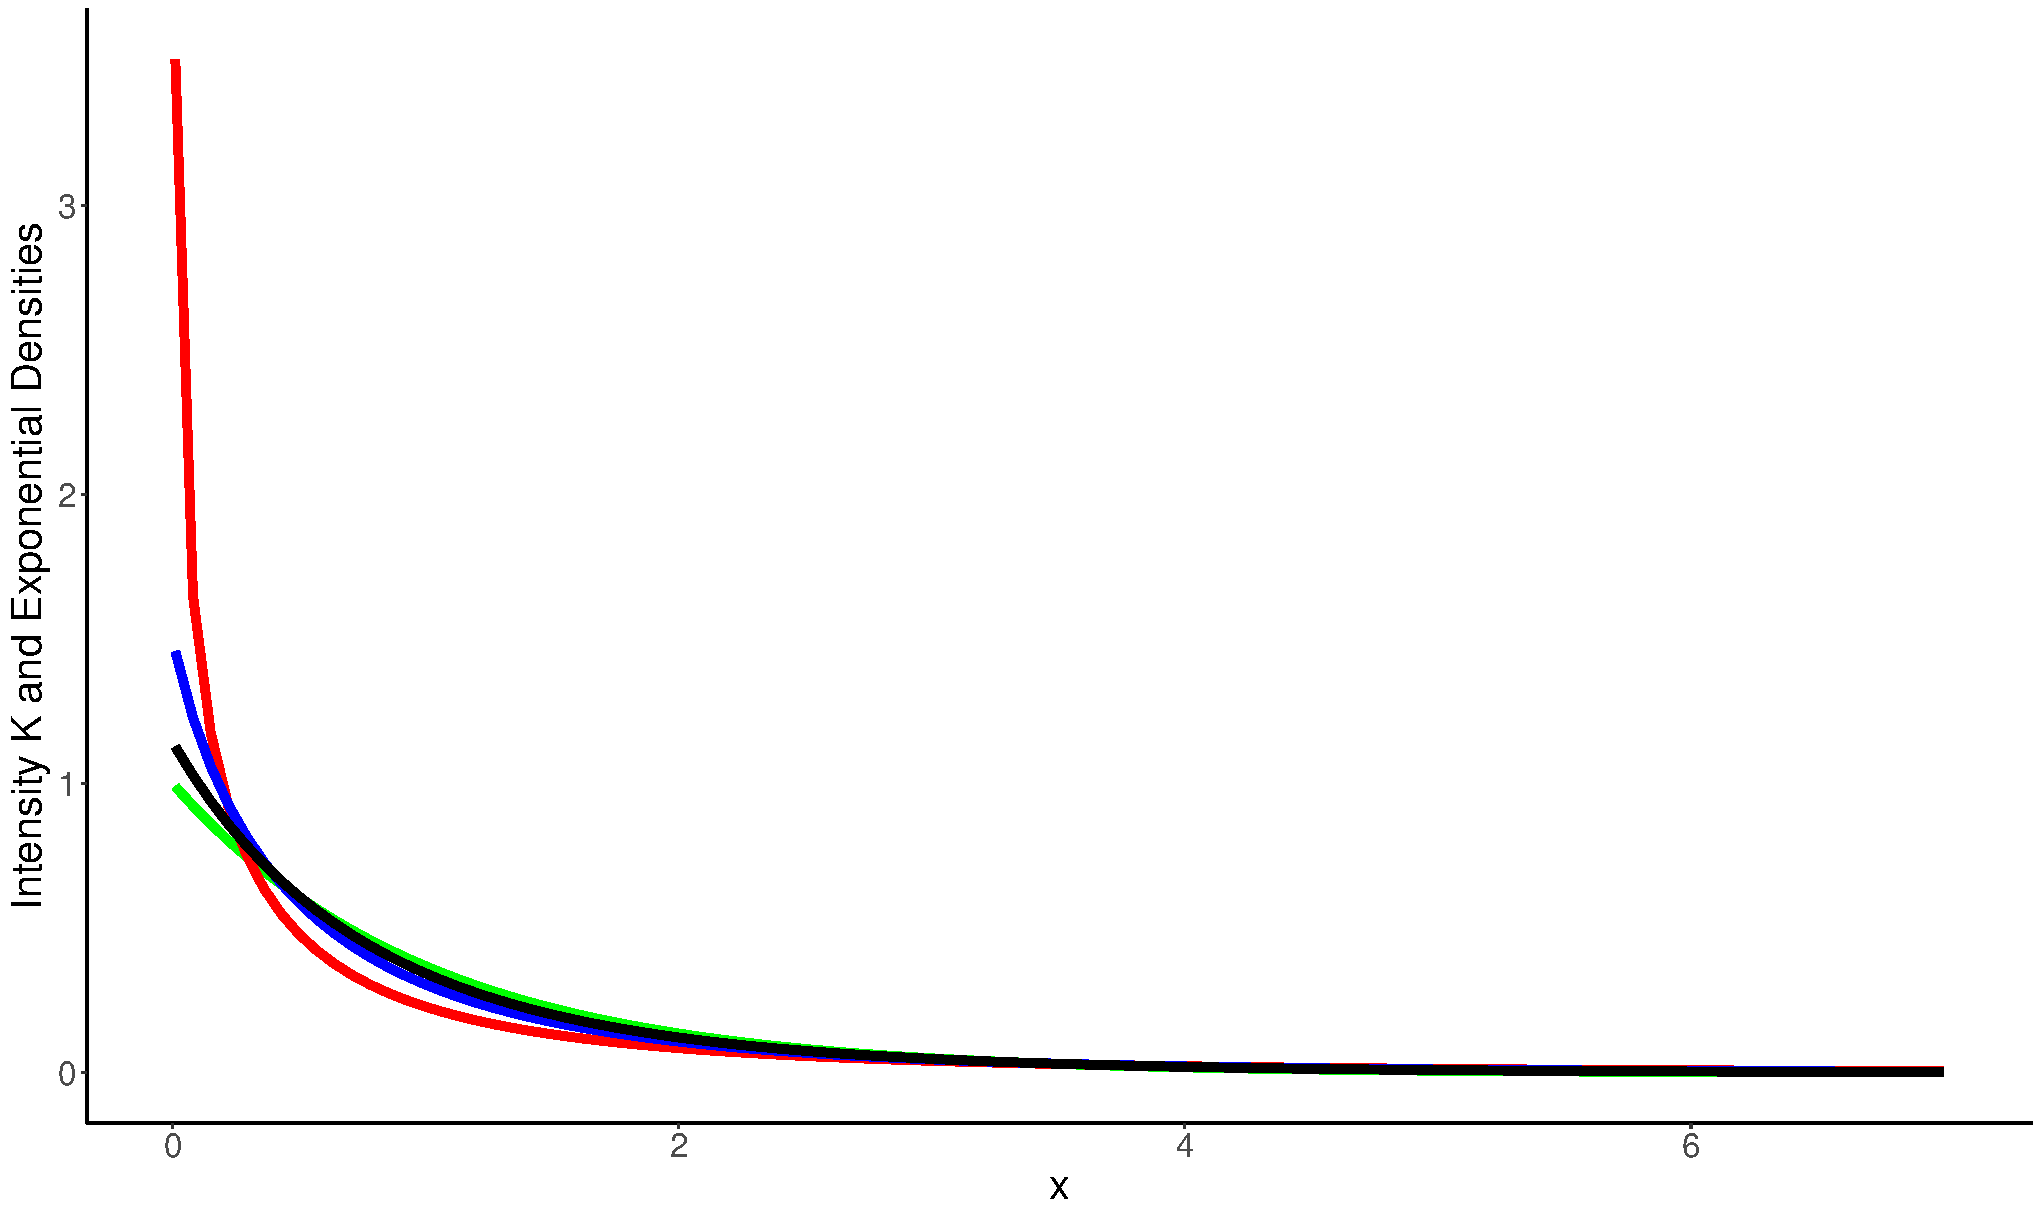
\includegraphics[width=.48\linewidth]{KIDensities}}
\subfloat[Densities in semilog scale\label{Fig:DensKISemilog}]{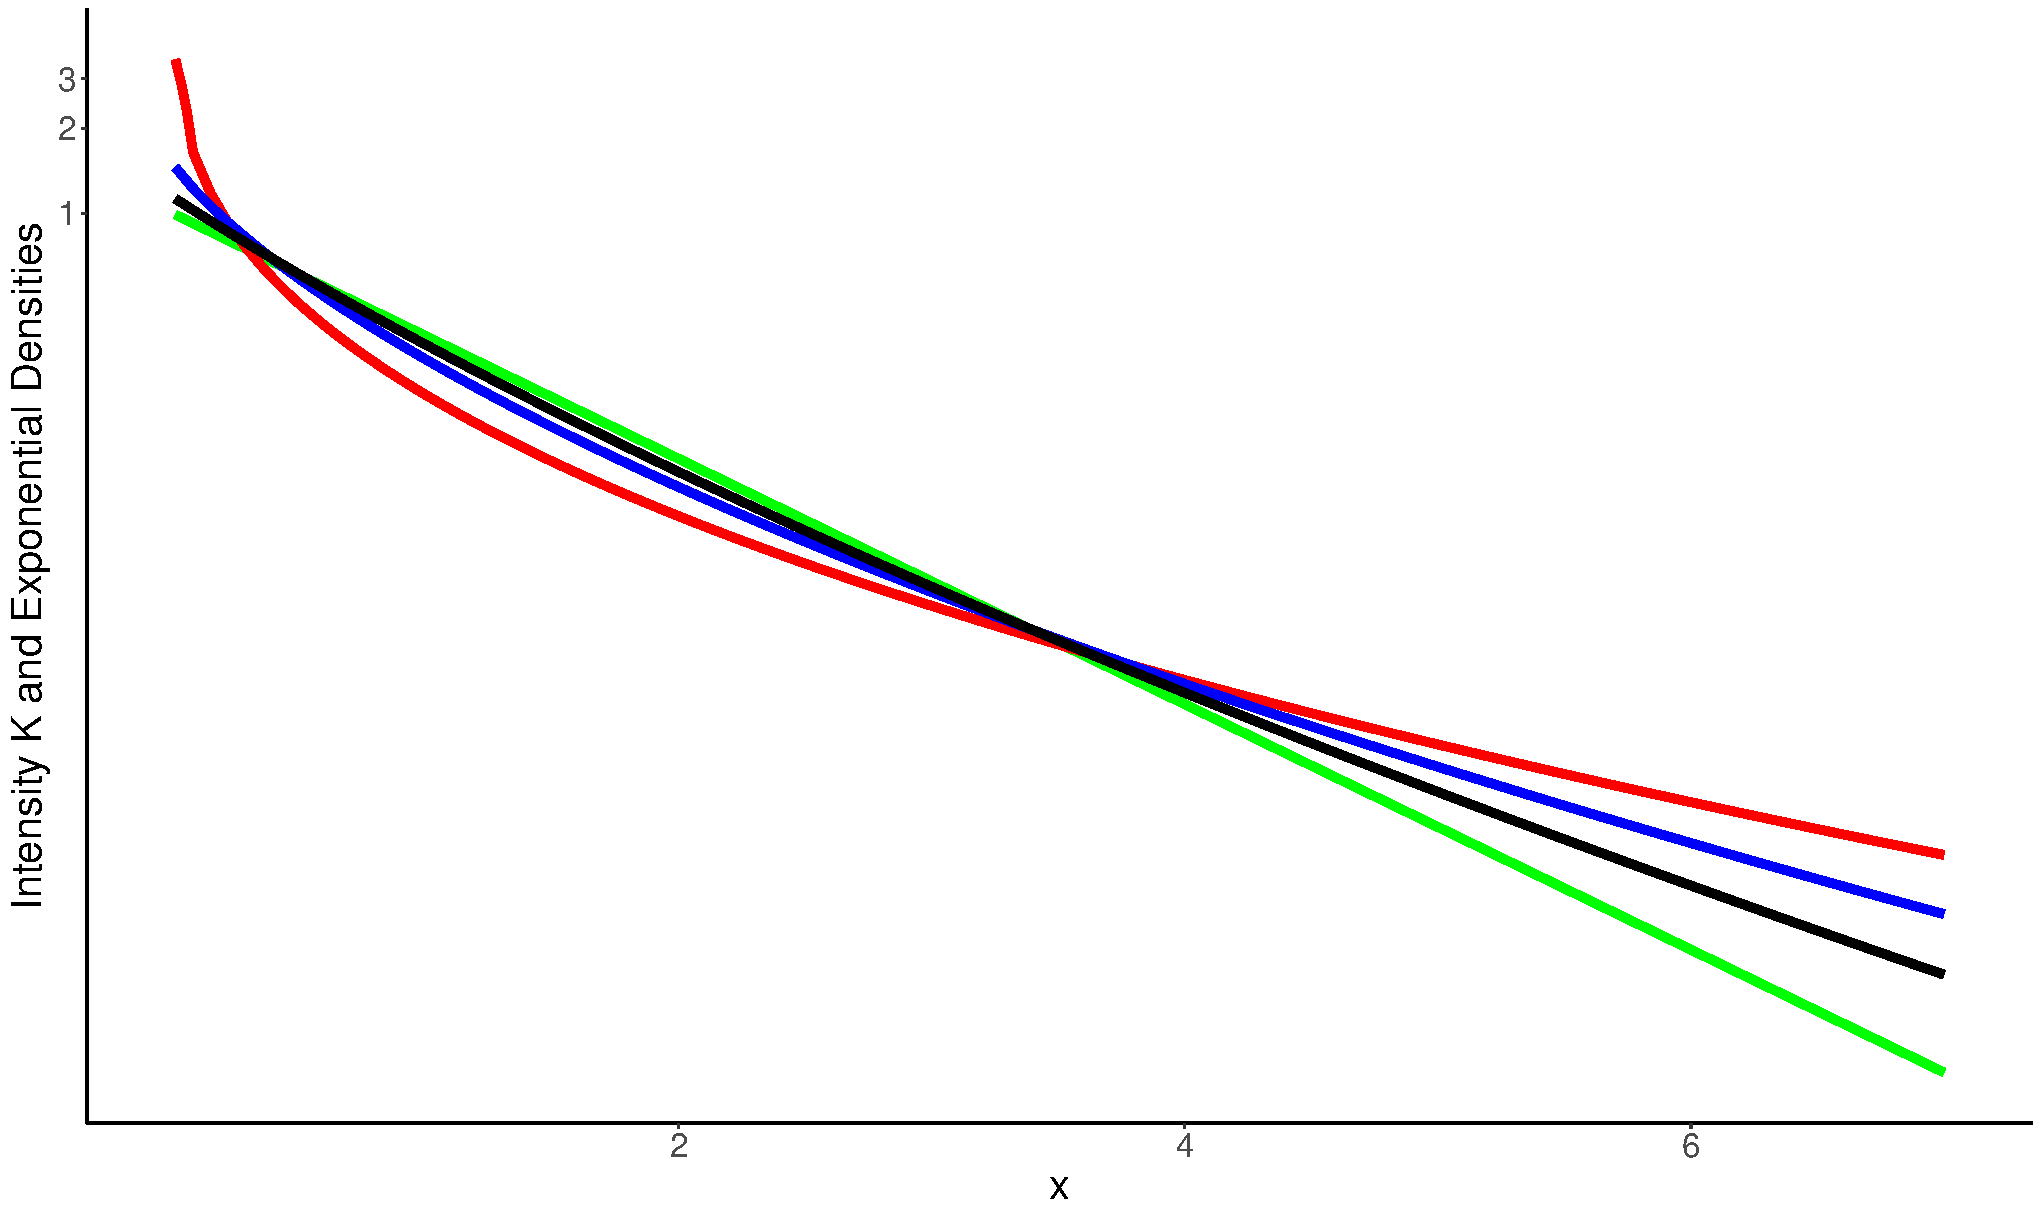
\includegraphics[width=.48\linewidth]{KIDensitiesSemilog}}
\caption[Densities in linear and semilogarithmic scale of the $\text{E}(1)$ (green) and $\mathcal K$ distributions]{Densities in linear and semilogarithmic scale of the $\text{E}(1)$ (green) and $\mathcal K$ distributions with unitary mean ($\alpha\in\{1,3,8\}$ in red, blue, and black, resp.)}\label{Fig:KIDistribution}
\end{figure}

The difference between these distributions is noteworthy, c.f.\ Fig.~\ref{Fig:KIDistribution}\subref{Fig:DensKISemilog}.
The green straight line is the density of the Exponential distribution, while the red one is that of the $\mathcal K(1,1,1)$ law.
The latter assigns larger probabilities to both small and large values, when compared with the former.
This leads, as will be seen later, to very contrasted data.

Fig.~\ref{Fig:KIDistributionLooks} shows the effect of varying the number of looks, for the same $\alpha=2$ and $\lambda=2$.

\begin{figure}[hbt]
\centering
\subfloat[Densities]{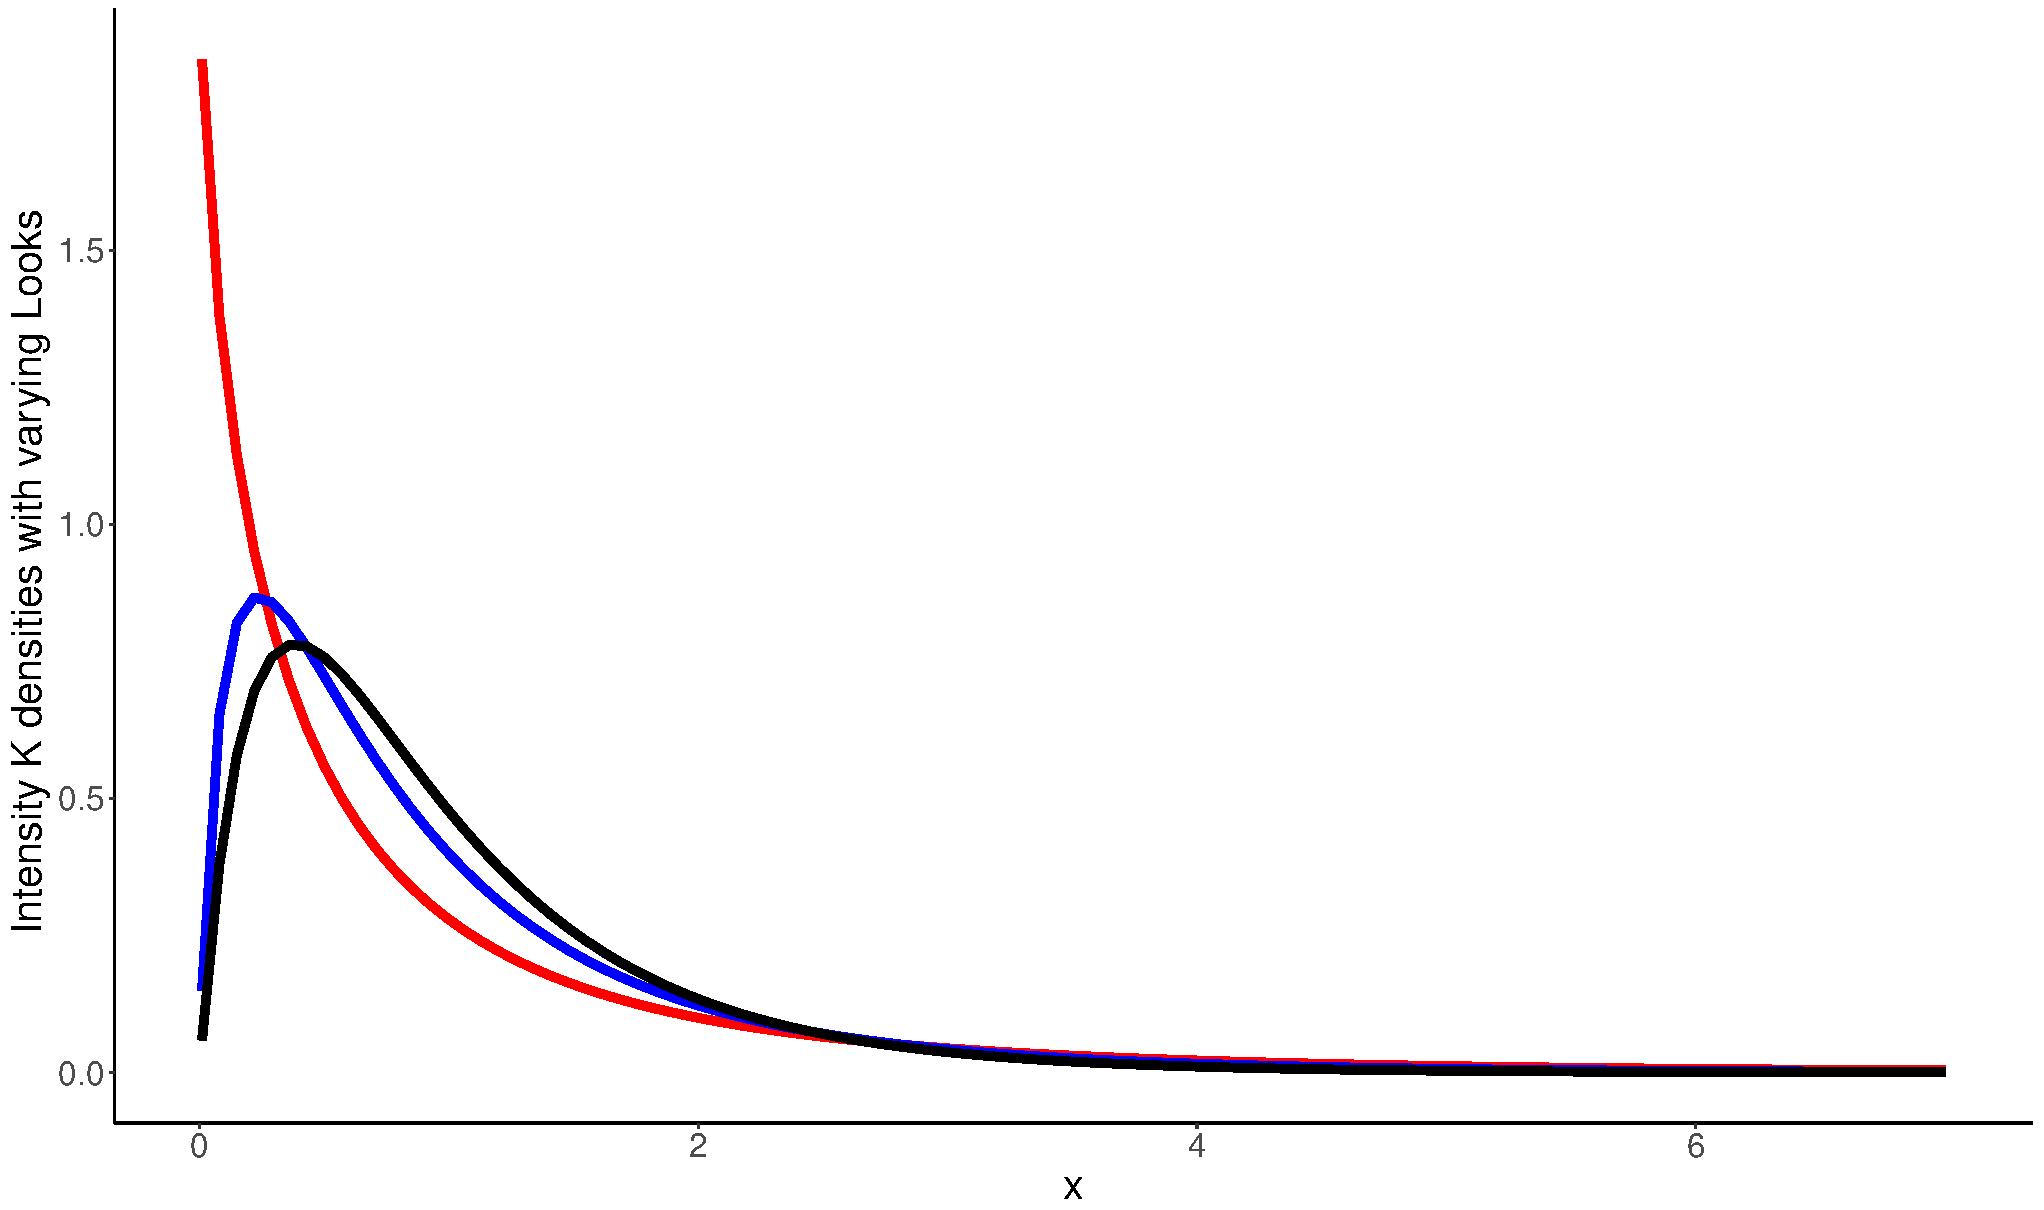
\includegraphics[width=.48\linewidth]{KIDensitiesLooks}}
\subfloat[Densities in semilog scale\label{KIDensitiesSemilog}]{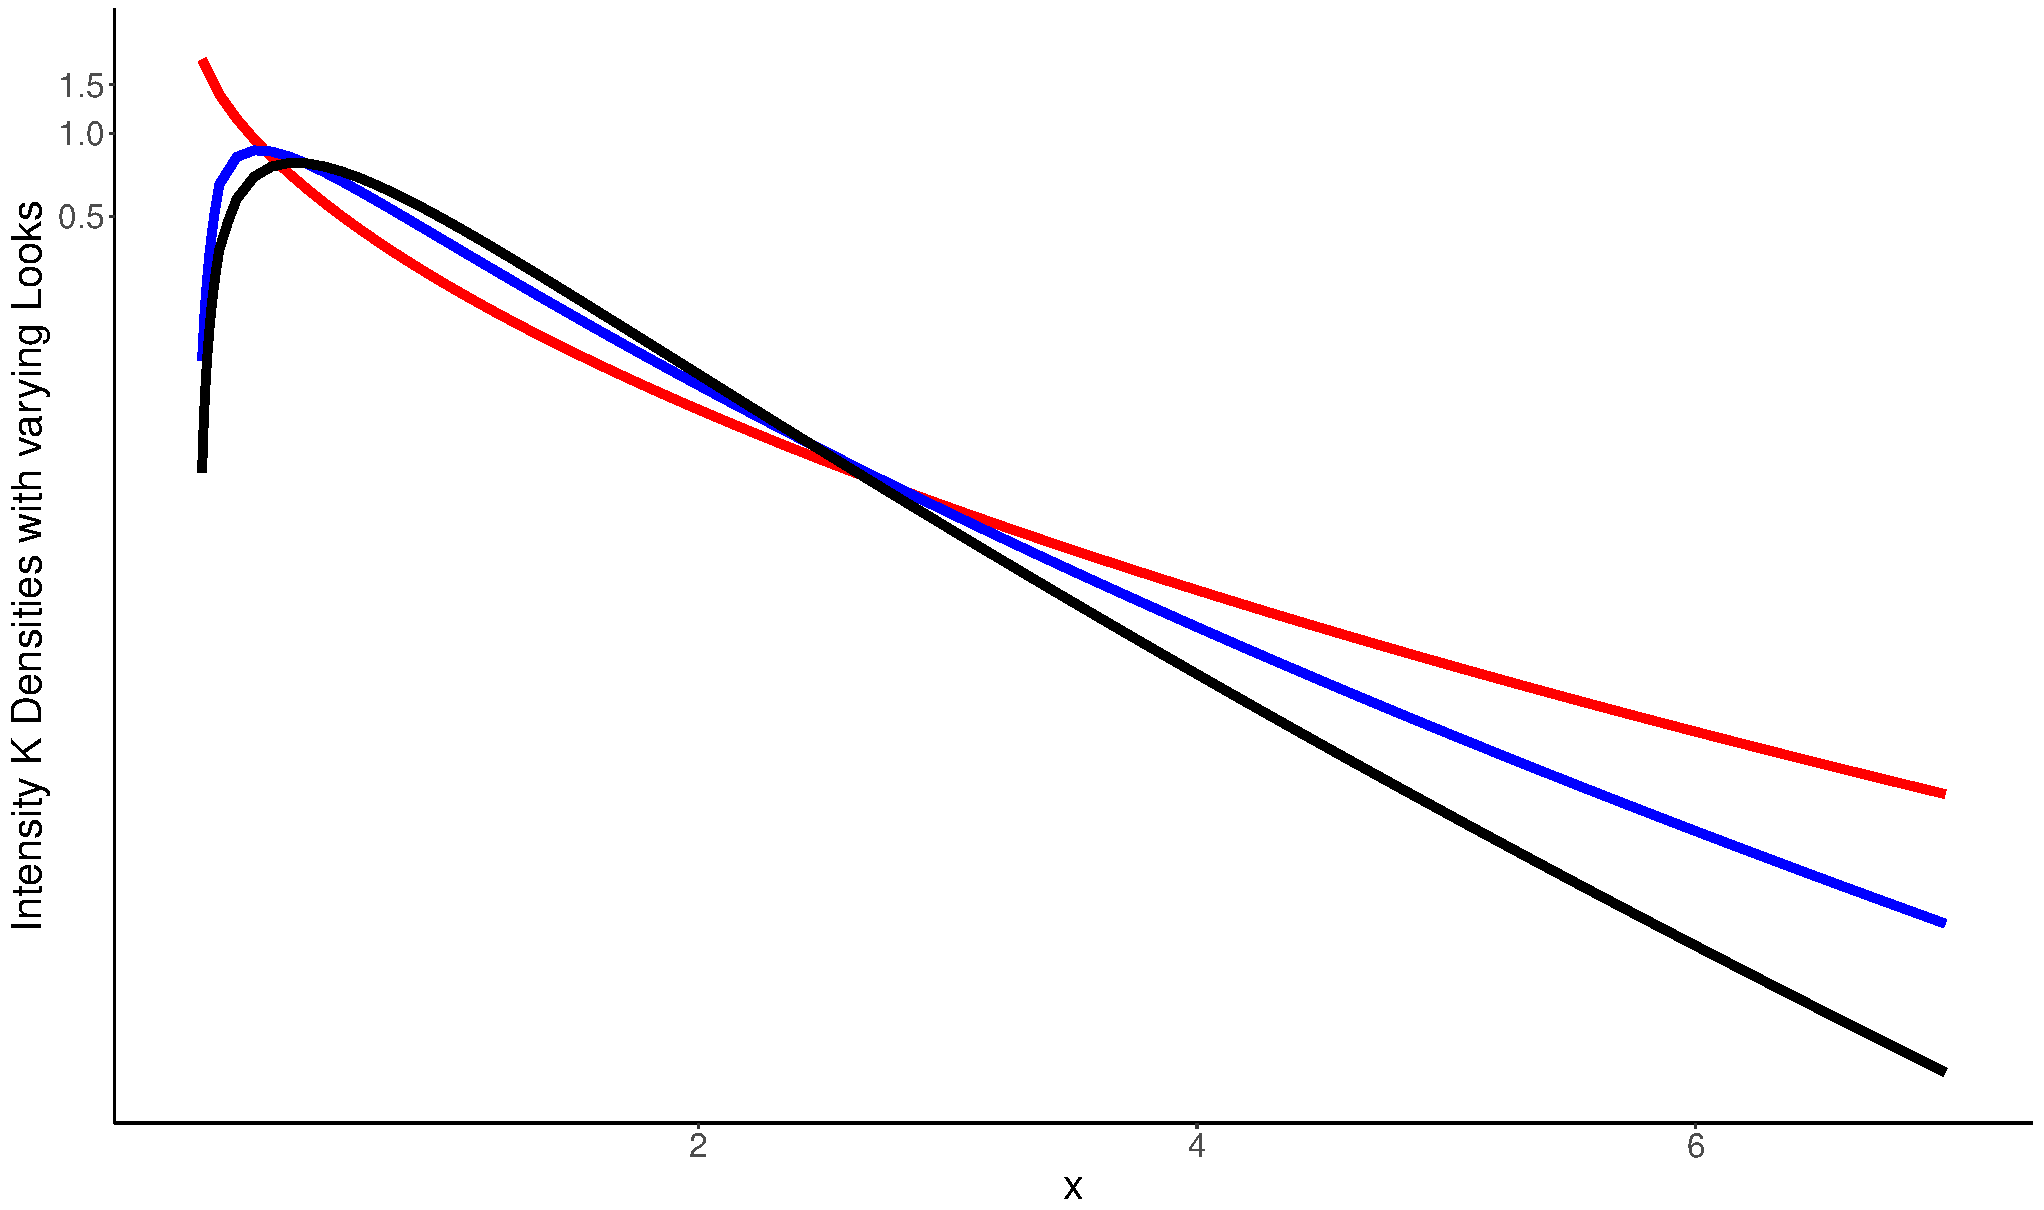
\includegraphics[width=.48\linewidth]{KIDensitiesSemilogLooks}}
\caption[Densities in linear and semilogarithmic scale $\mathcal K(2,2,L)$ distributions with unitary mean and $L\in\{1,3,8\}$]{Densities in linear and semilogarithmic scale $\mathcal K(2,2,L)$ distributions with unitary mean and $L\in\{1,3,8\}$ in red, blue, and black, resp.)}\label{Fig:KIDistributionLooks}
\end{figure}

Notice in Fig~\ref{Fig:KIDistributionLooks}\subref{KIDensitiesSemilog} the dramatic effect multilook processing has mostly on the distribution of very small values.
This, along with the reduced probability very large values have with multilook processing, yields less contrasted images.

Although the basic construction, and physical explanation, of the $\mathcal K$ distribution stems from letting fluctuate the number of elementary backscatters, we are interested in an equivalent derivation.

As previously said, the basic model for observations without roughness is~\eqref{eq:SARGammaDensity}.
The mean $X=\sigma^2$ can be seen as multiplying $Y$, a $\Gamma(1,L)$ random variable, which describes the speckle.
As we are interested in letting the mean fluctuate, $X$ can be described by any distribution with positive support.
If we choose a Gamma random variable with mean $\alpha/\lambda>0$ and shape parameter $\alpha>0$, i.e., $Y\sim\Gamma(\alpha/\lambda,\alpha)$, and further assume that $X$ and $Y$ are independent, then the product $Z=XY$ follows a $\mathcal{K}(\alpha,\lambda,L)$ distribution with density~\eqref{Eq:DensKI}.
This \textit{multiplicative} construction is not only useful for sampling from this distribution, but also for obtaining other models for the return.

\section{The $\mathcal G^0$ distribution}

In this line, \citet{frery96} noticed that the $\mathcal{K}$ distribution failed at describing data from extremely textured areas as, for instance, urban targets.
The authors then proposed a different model for the backscatter $X$: the Reciprocal Gamma distribution.

We say that $X\sim{\Gamma^{-1}}(\alpha,\gamma)$, with $\alpha<0$ and $\gamma>0$ follows a 
Reciprocal Gamma distribution is characterized by the density
\begin{equation}
f_X(x;\alpha,\gamma) = \frac{1}{\gamma^\alpha} x^{\alpha-1} \exp\{-\gamma/x\},
\label{Eq:IGdensity}
\end{equation}
for $x>0$ and zero otherwise.

Now introducing the Reciprocal Gamma model for the backscatter in the multiplicative model, i.e. by multiplying the independent random variables $X\sim{\Gamma^{-1}}(\alpha,\gamma)$ and $Y\sim\Gamma(1,L)$, one obtains the $\mathcal{G}^0$ distribution for the return $Z=XY$, which is characterized by the density
\begin{equation}
f_Z(z; \alpha,\gamma,L) = \frac{L^L \Gamma(L-\alpha)}{\gamma^\alpha \Gamma(L)\Gamma(-\alpha)} \frac{z^{L-1}}{(\gamma+L z)^{L-\alpha}},
\label{Eq:DensGI0}
\end{equation}
where $\alpha<0$, and $\gamma,z>0$.
It is noteworthy that, differently from~\eqref{Eq:DensKI}, this density does not involve Bessel functions.

We denote $Z\sim \mathcal G^0(\alpha,\gamma,L)$ the situation of $Z$ following the distribution characterized by~\eqref{Eq:DensGI0}.
The $k$-order moments of $Z$ are
\begin{equation}
E(Z^k) = (\gamma / L)^{k} \frac{\Gamma(L+k)\Gamma(-\alpha-k)}{\Gamma(L)\Gamma(-\alpha)},
\label{Eq:MomentGI0}
\end{equation}
provided $-\alpha>k$, and infinite otherwise.
Eq.~\eqref{Eq:MomentGI0} is useful, among other applications, for finding $\gamma^*=-\alpha-1$, the scale parameter that yields a unitary mean distribution for each $\alpha$ and any $L$.

Fig.~\ref{Fig:GI0Distribution} shows the $\text{E}(1)$ and $\mathcal G^0(\alpha,\gamma^*, 1)$ densities.
The differences in tail behavior are clearly exhibited in the semilogarithmic scale; cf.\ Fig.~\ref{Fig:GI0Distribution}\subref{Fig:DensGI0Semilog}.
Whereas the exponential distribution decreases linearly, the $\mathcal G^0$ law assigns more probability to larger events increasing, thus, the variability of the return.

\begin{figure}[hbt]
\centering
\subfloat[Densities]{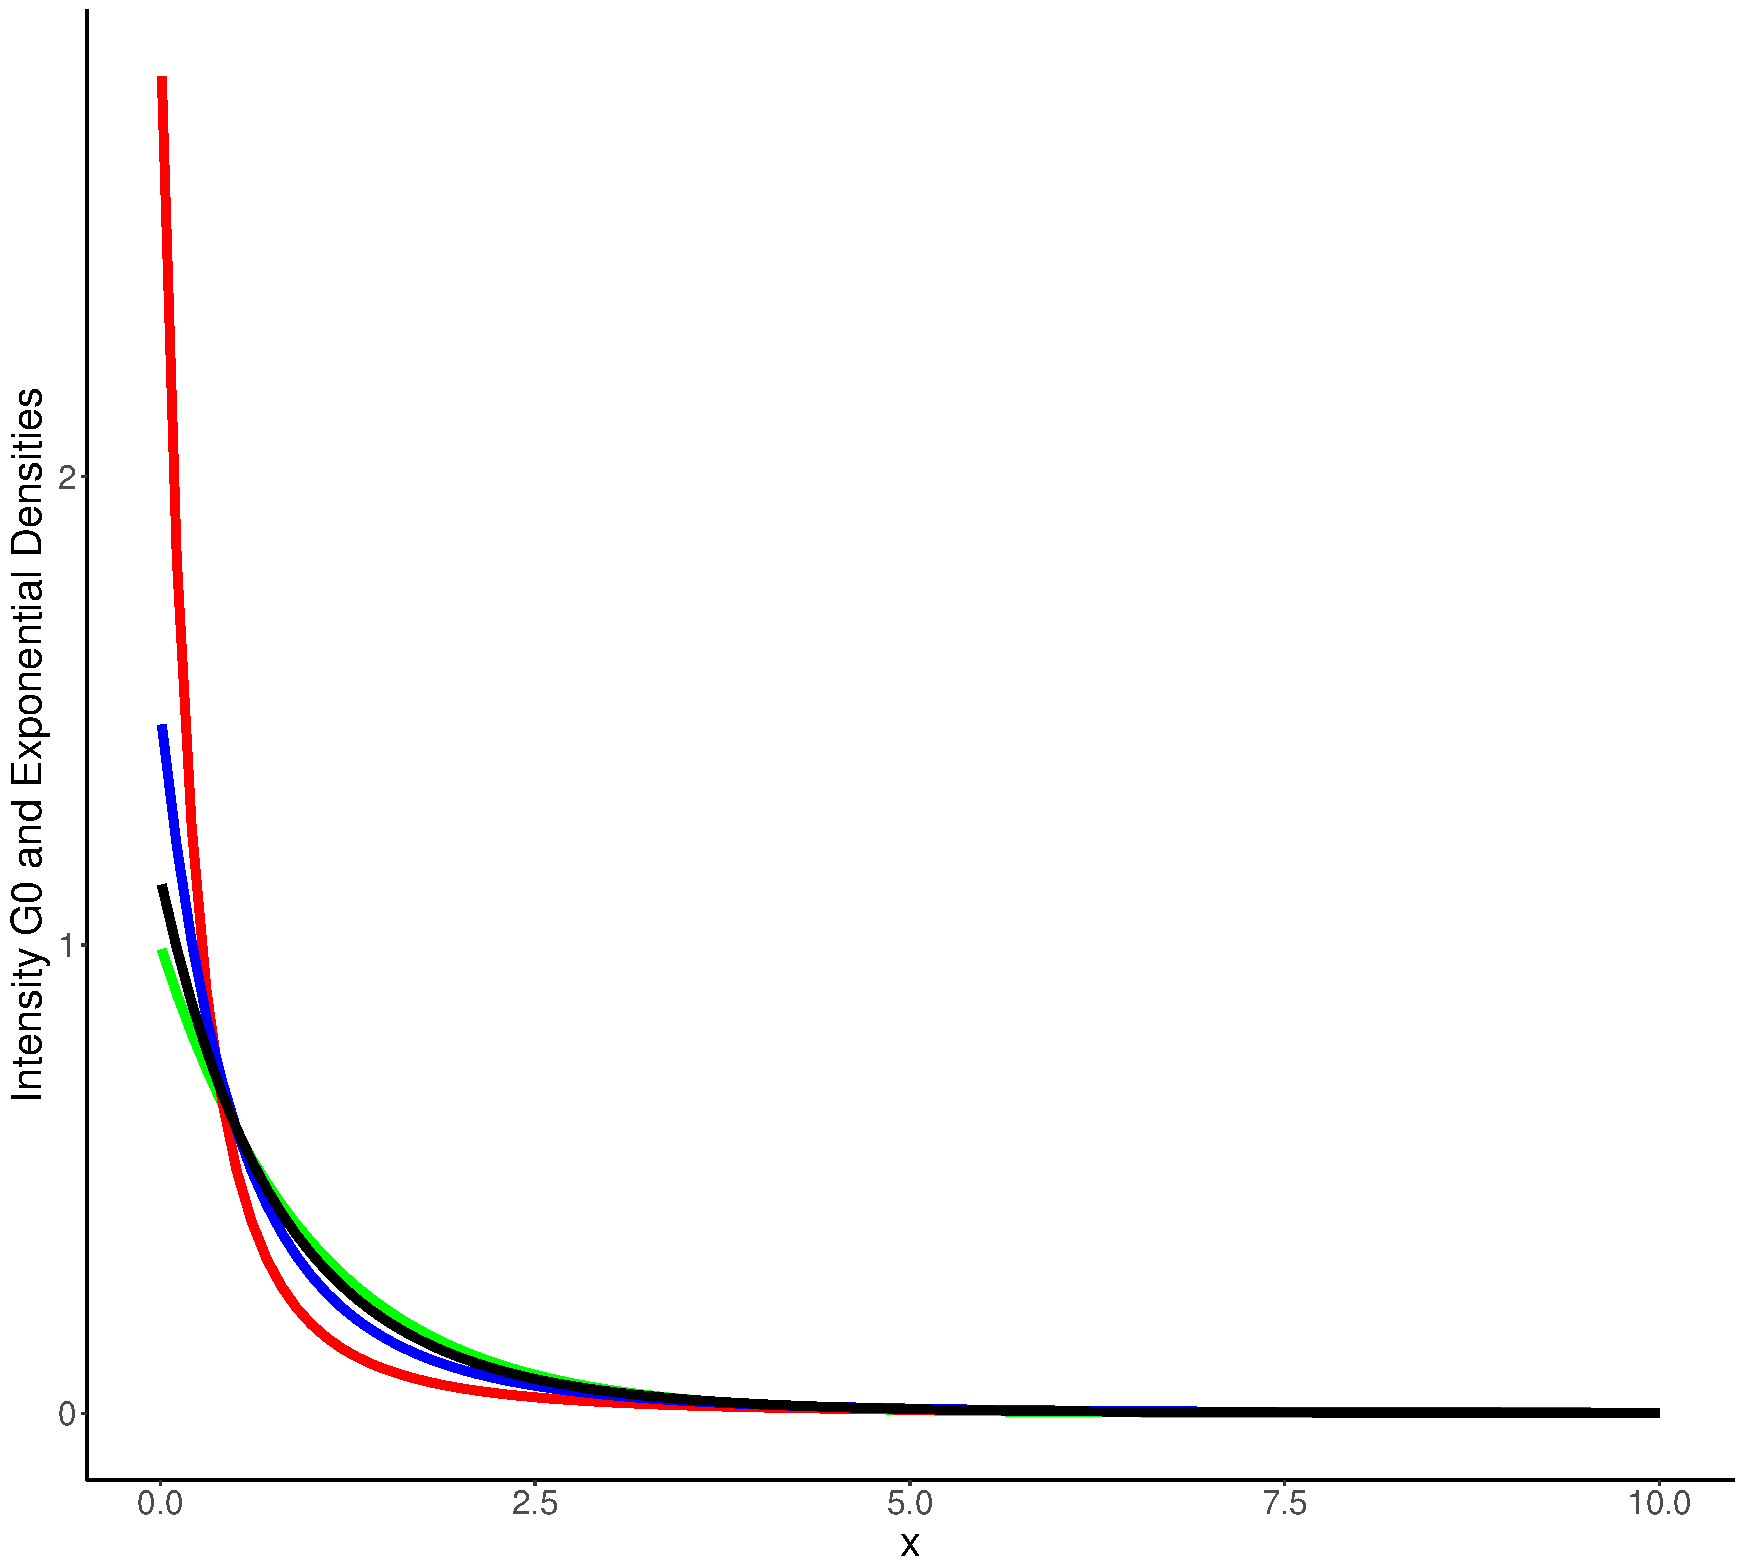
\includegraphics[width=.48\linewidth]{GI0Densities}}
\subfloat[Densities in semilog scale\label{Fig:DensGI0Semilog}]{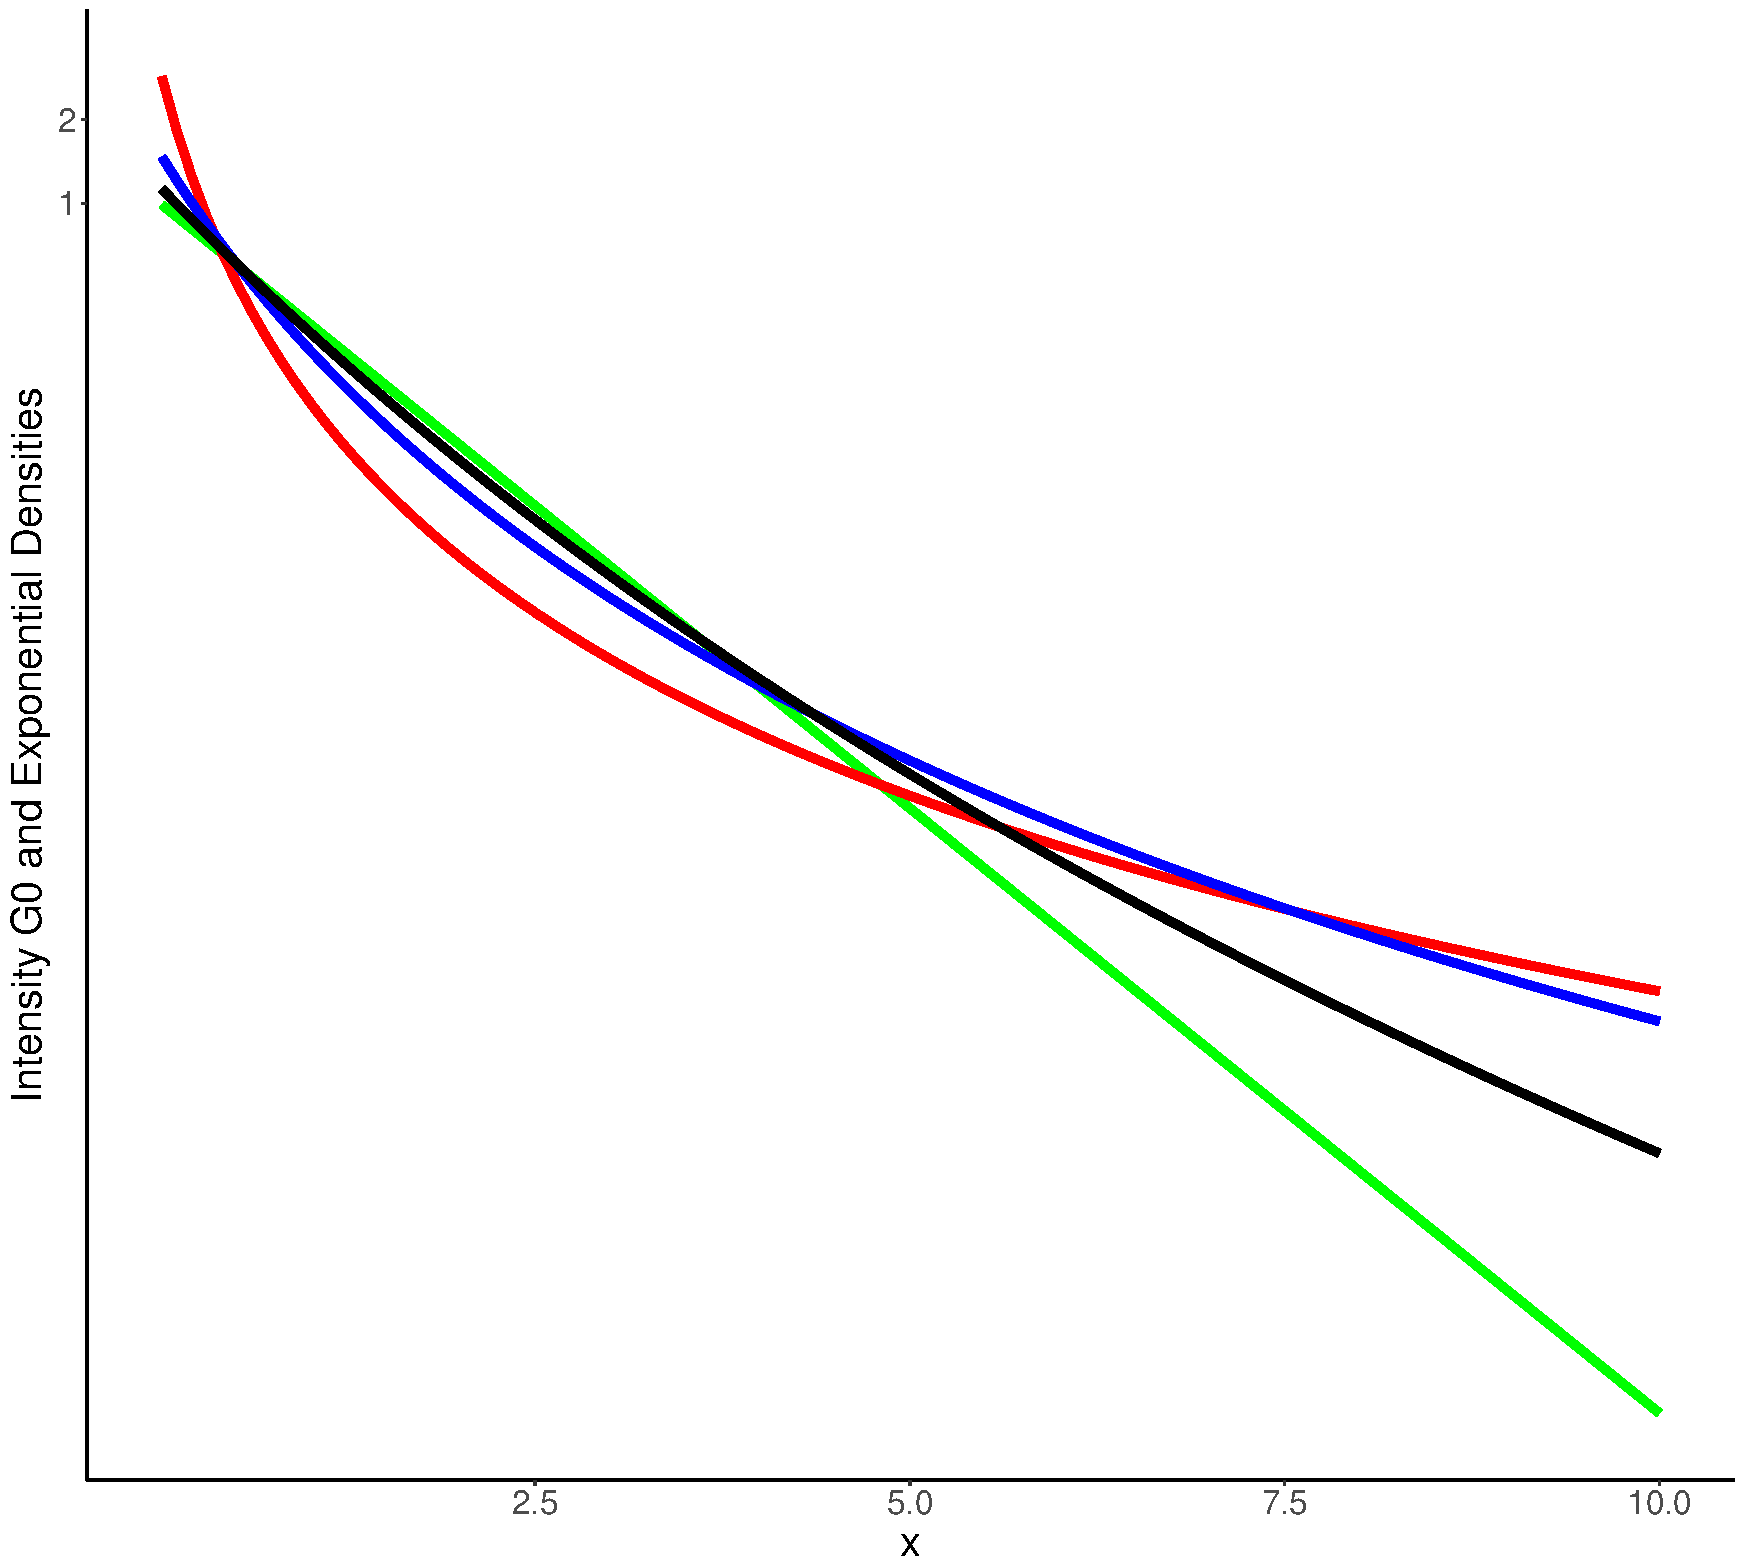
\includegraphics[width=.48\linewidth]{GI0DensitiesSemilog}}
\caption[Densities in linear and semilogarithmic scale of the $\text{E}(1)$ (green) and $\mathcal G^0$ distributions with unitary mean]{Densities in linear and semilogarithmic scale of the $\text{E}(1)$ (green) and $\mathcal G^0$ distributions with unitary mean and $\alpha\in\{-1.5,-3,-8\}$ in red, blue, and black, resp.}\label{Fig:GI0Distribution}
\end{figure}

Fig.~\ref{Fig:GI0DistributionLooks} shows the effect of varying the number of looks, for the same $\alpha=5$ and $\gamma=4$.

Notice, again, in Fig~\ref{Fig:GI0DistributionLooks}\subref{GI0DensitiesSemilog} the effect multilook processing has mostly on the distribution of very small values.
This, along with the reduced probability very large values have with multilook processing, yields less contrasted images.

\begin{figure}[hbt]
\centering
\subfloat[Densities]{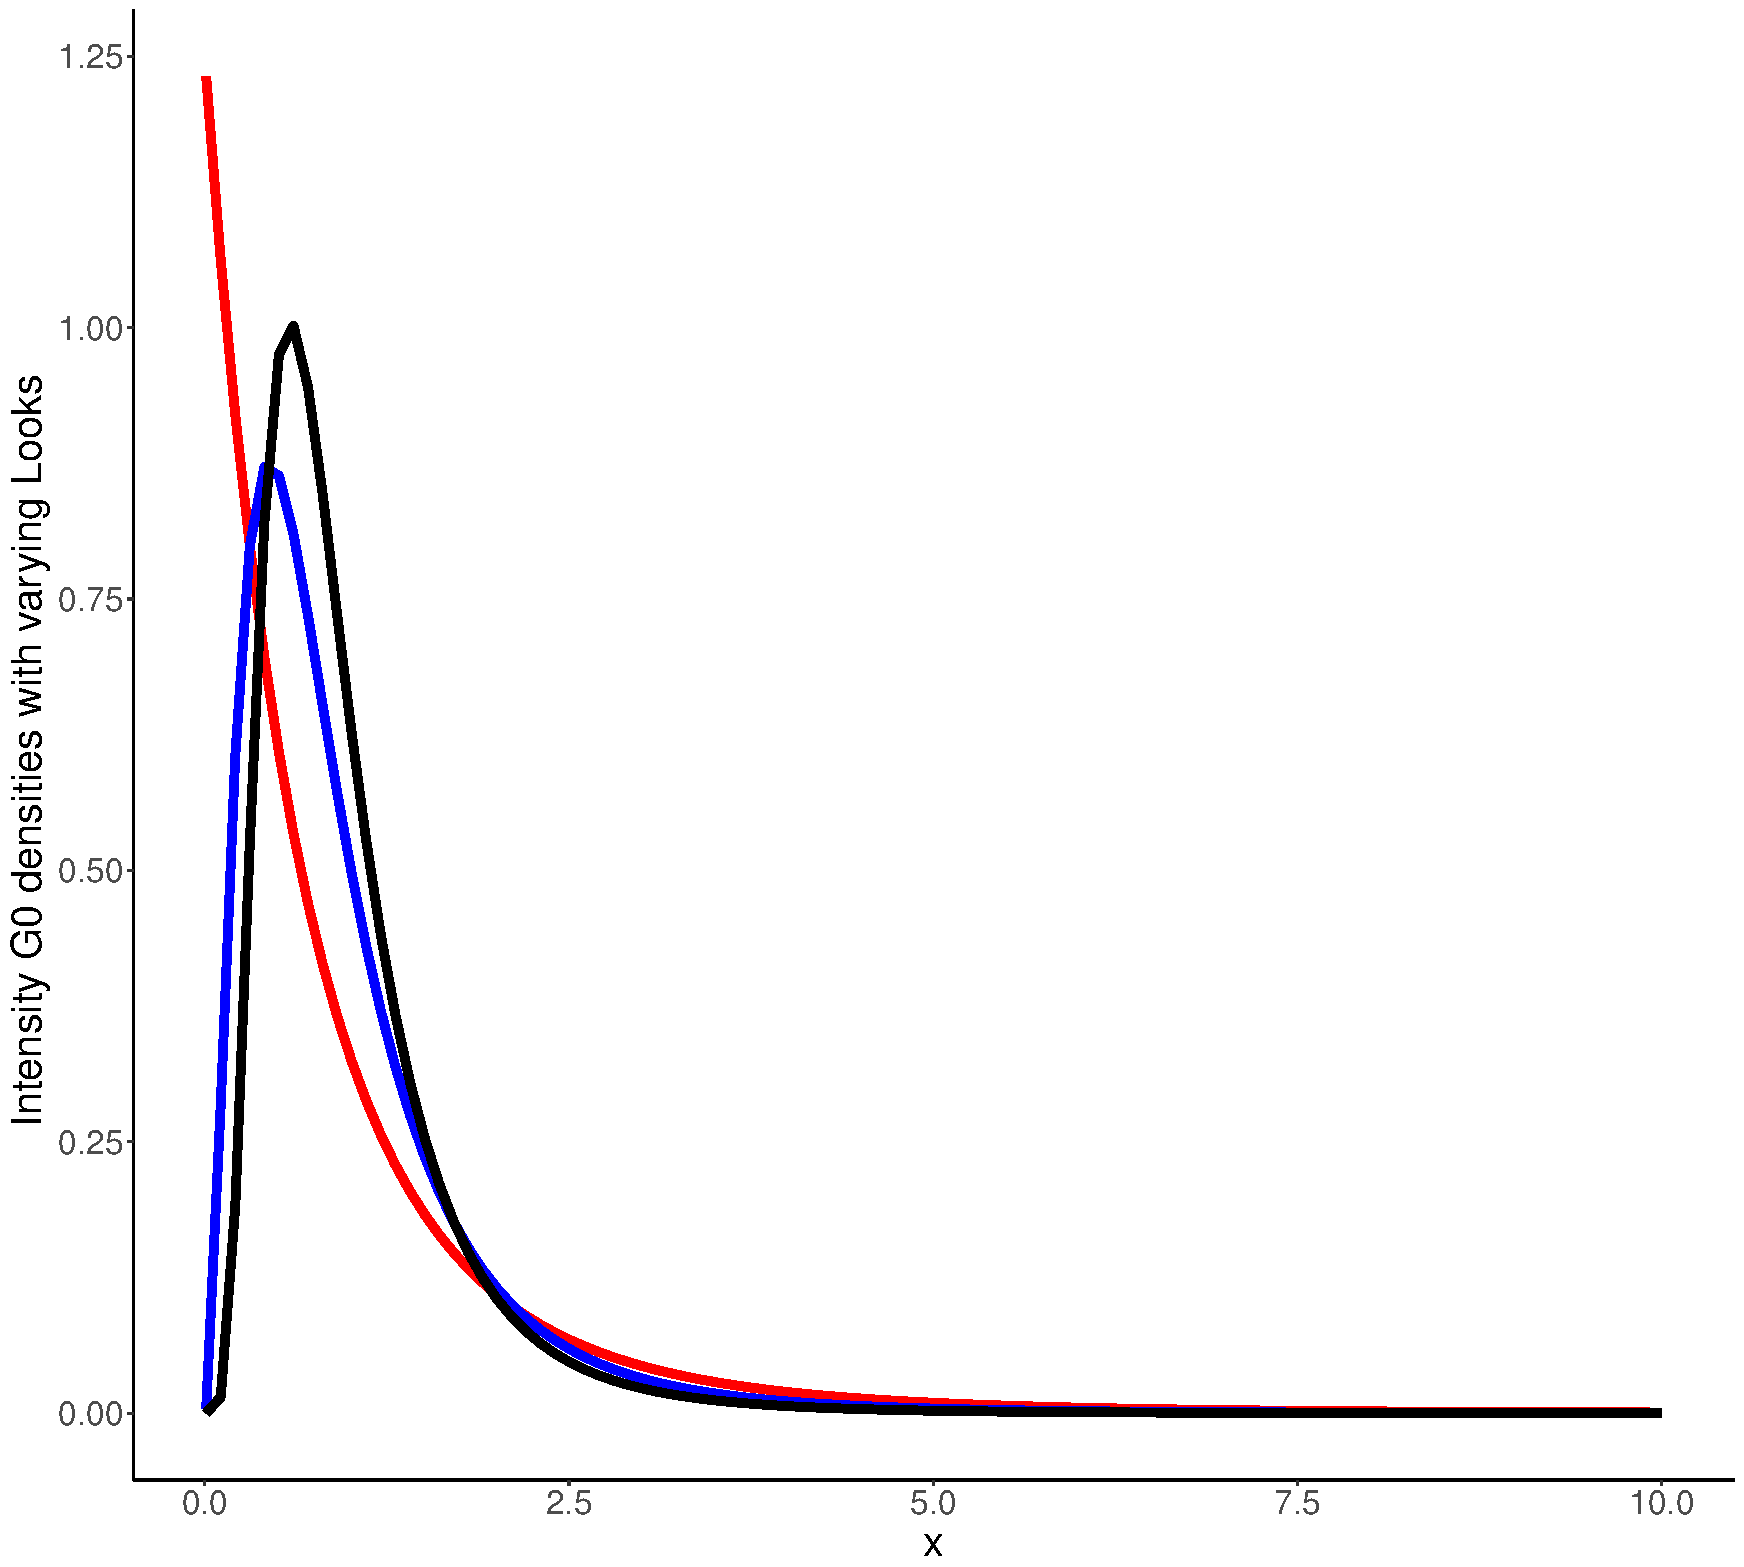
\includegraphics[width=.48\linewidth]{GI0DensitiesLooks}}
\subfloat[Densities in semilog scale\label{GI0DensitiesSemilog}]{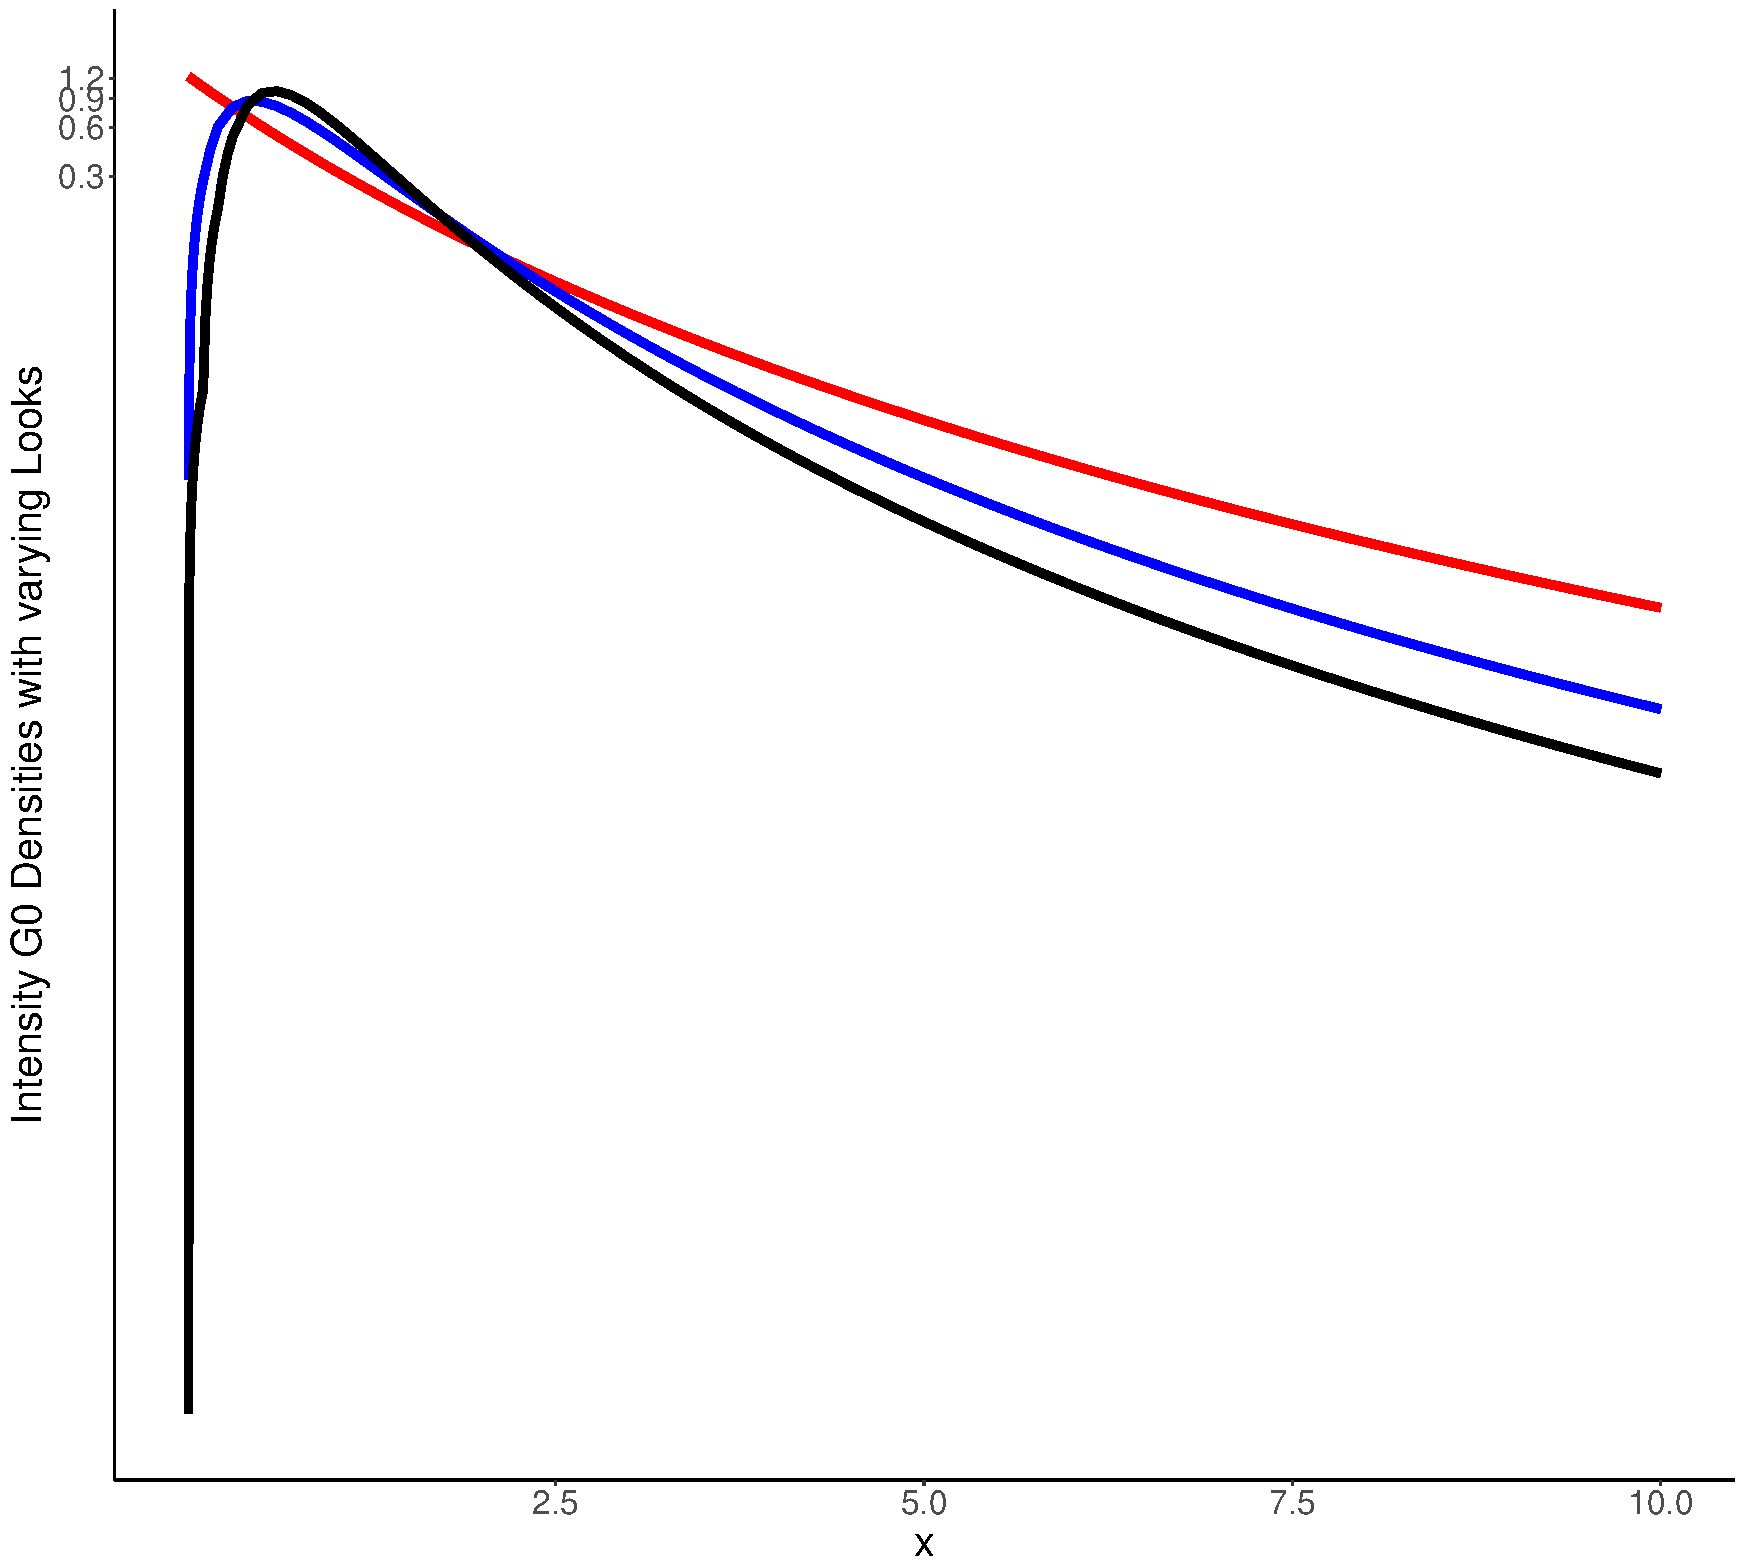
\includegraphics[width=.48\linewidth]{GI0DensitiesSemilogLooks}}
\caption[Densities in linear and semilogarithmic scale $\mathcal G^0(-5,4,L)$ distributions with unitary mean and $L\in\{1,3,8\}$]{Densities in linear and semilogarithmic scale $\mathcal G^0(-5,4,L)$ distributions with unitary mean and $L\in\{1,3,8\}$ in red, blue, and black, resp.)}\label{Fig:GI0DistributionLooks}
\end{figure}

The $\mathcal{G}^0$ distribution has the same number of parameters as the $\mathcal{K}$ law, but it has been shown to be more apt at modeling return with extreme variability.
Moreover, it is also able to describe the same kind of return from textured areas for which the latter was proposed; \citet{MejailJacoboFreryBustos:IJRS} showed that, with proper choices of parameters, the $\mathcal G^0$ law can approximate with any error any $\mathcal K$ distribution.
For these reasons, the $\mathcal G^0$ distribution is called \textit{Universal Model} for SAR data; see Exercise~\ref{Ex:ApproximationKGI0}.

The $\mathcal G^0$ distribution relates to the well-known Fisher-Snedekor law in the following manner:
\begin{equation}
F_{G^0(\alpha,\gamma,L)}(t) = \Upsilon_{2L,- 2\alpha}(- \alpha t/\gamma),
\end{equation}
where $\Upsilon_{u,v}$ is the cumulative distribution function of a Fisher-Snedekor distribution with $u$ and $v$ degrees of freedom, and $F_{G^0(\alpha,\gamma,L)}$ is the cumulative distribution function of a $F_{G^0(\alpha,\gamma,L)}$ random variable.
Notice that $\Upsilon$ is readily available in most software platforms for statistical computing.
Since such platforms usually also provide implementations of the inverse of cumulative distribution functions, the Inversion Theorem can be used to sample from the $\mathcal G^0$ law.

Arguably, the most popular way of sampling from the $\mathcal G^0$ distribution is through its multiplicative nature.
Obtaining deviates from $X\sim\Gamma(1,L)$ is immediate.
In order to sample from $Y\sim\Gamma^{-1}(\alpha,\gamma)$, one may use the fact that if $Y'\sim\Gamma(-\alpha,\gamma)$, then $Y=1/Y'$ has $\Gamma^{-1}(\alpha,\gamma)$ distribution.
Then, $Z=X/Y'$ has the desired $\mathcal G^0(\alpha,\gamma,L)$ distribution.

\citet{IGARSSChan2017} discuss other techniques for obtaining such deviates, in particular interesting connections between the $\mathcal G^0(\alpha,\gamma,1)$ law and certain Pareto distribution.

\section{Connection between Models}

\section*{Exercises}

\begin{exer}
Using~\eqref{Eq:MomentKI}, compute the skewness and kurtosis of the $\mathcal K(\alpha,\lambda,L)$ distribution.
Illustrate how they vary with the parameters.
\end{exer}

\begin{exer}
Illustrate the dependence of the density of the $\mathcal K$ distribution with respect to the scale parameter $\lambda$.
\end{exer}

\begin{exer}
Obtain samples from iid $\mathcal{K}(\alpha,\lambda,L)$ random variables.
Produce histograms, and draw the theoretical densities over them for a variety of parameters.
\end{exer}

\begin{exer}
Obtain the expression of the density of $\mathcal K$-distributed amplitude data via the transformation $Z_A=\sqrt{Z_I}$.
Compute its moments.
Illustrate.
\end{exer}

\begin{exer}
Using~\eqref{Eq:MomentGI0}, compute the skewness and kurtosis of the $\mathcal G^0(\alpha,\gamma,L)$ distribution.
Illustrate how they vary with the parameters.
\end{exer}

\begin{exer}
Illustrate the dependence of the density of the $\mathcal G^0$ distribution with respect to the scale parameter $\gamma$.
\end{exer}

\begin{exer}
Obtain samples from iid $\mathcal{G}^0(\alpha,\gamma,L)$ random variables.
Produce histograms, and draw the theoretical densities over them for a variety of parameters.
\end{exer}

\begin{exer}
Obtain the expression of the density of $\mathcal G^0$-distributed amplitude data via the transformation $Z_A=\sqrt{Z_I}$.
Compute its moments.
Illustrate.
\end{exer}

\begin{exer}
Consider~\eqref{Eq:DensGI0} and~\eqref{Eq:MomentGI0}.
Computer $\mu$, the expected value, from the latter, and reparametrize the former using $\mu$, $\alpha$, and $L$.
\end{exer}

\begin{exer}\label{Ex:ApproximationKGI0}
Propose a measure of the difference between $Z_1\sim\mathcal K(\alpha_1,\lambda^*, L)$ and $Z_2\sim\mathcal G^0(\alpha_2,\gamma^*, L)$ (consider, for instance, the Hellinger distance between distributions with positive support $d_{\text{H}}(Z_1,Z_2)=1-\int_{\mathbbm R_+}\sqrt{f_{Z_1} f_{Z_2}})$.
Describe this difference for a number of values of $\alpha_1$ and $\alpha_2$, for $L\in\{1,3,8\}$.
For each $\alpha_1$, find the value of $\alpha_2$ which yields the closest $\mathcal K$ and $\mathcal G^0$ random variables\cite{mejailfreryjacobobustos2001}.
\end{exer}
